\section{Dungeon Generierung mittels Space Partitioning}\label{WG:SpacePartitioning}
In diesem Abschnitt wird eine Methode beschrieben Dungeons mithilfe von Space Partitioning prozedural zu generieren. Dungeons sind Level, die aus mehreren Räumen bestehen, die durch Korridore miteinander verbunden sind. Die Räume haben eine rechteckige Grundfläche, deren Breite und Tiefe durch Space Partitioning Algorithmen bestimmt sind. Das hier beschriebene Vorgehen orientiert sich an dem Buch \textit{Procedural Content Creation in Games} \cite{Shaker2016}.

\subsection{Space Partitioning}
Ein Space Partitioning Algorithmus unterteilt einen Raum in Partitionen. In der Regel handelt es sich bei den Ausgangsräumen um zwei- oder dreidimensionale Räume. Hier wird angenommen, dass der zu partitionierende Raum eine rechteckige (zweidimensionale) Fläche ist. Die Partitionierung der Räume erfolgt mithilfe von $k$-d-Bäumen oder Quadtrees. Beide Algorithmen speichern die Partitionierung des Raumes in einer Baumstruktur und arbeiten rekursiv.

Bei der Partitionierung eines zweidimensionalen Raumes mit einem $k$-d-Baum wird in jedem Schritt eine Achse zufällig ausgewählt, an der die Eingabefläche in zwei Teile partitioniert wird. Anschließend wird ein Punkt ausgewählt, der die Grenze zwischen den beiden Partitionen bestimmt. Dabei stellt die Eingabefläche einen Knoten im Baum dar, an den zwei Kindknoten für die Partitionen angehangen werden. So entsteht ein Binärbaum, in dem die Wurzel die Ausgangsfläche enthält und ein innerer Knoten oder Blattknoten eine der zwei Partitionen des Elternknotens enthält. Der Algorithmus wird so lange rekursiv angewandt, bis ein Abbruchkriterium erfüllt ist. Als Abbruchkriterium kann z.B. eine minimale Größe einer Partition gefordert werden. Alternativ kann die Höhe des Baumes durch einen maximalen Wert beschränkt werden. Die Blätter des Baumes enthalten die Partitionen der Ausgangsfläche. Abbildung \ref{04spdgkdtree} illustriert die Partitionierung einer quadratischen Fläche mit einem $k$-d-Baum. Als Abbruchkriterium wurde hier eine minimale Größe der Partitionen gewählt, daher wurden die Partitionen $4$ und $5$ nicht weiter unterteilt und der Baum ist nicht vollständig. 

\begin{figure}[h]
\centering
\begin{tabular}{cc}
    \begin{minipage}{.4\textwidth}
      \begin{center}
      \textbf{Raum}
      \end{center}
    \begin{center}
    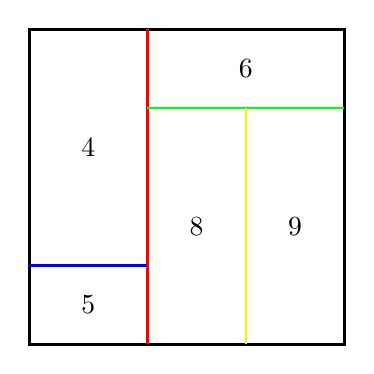
\begin{tikzpicture}  
      \draw[very thick] (2,-2) rectangle (6,2);
  
      \draw[thick, red] (3.5,-2) -- (3.5,2);
      \draw[thick, blue] (2,-1) -- (3.5,-1);
      \draw[thick, green] (6,1) -- (3.5,1);
      \draw[thick, yellow] (4.75,1) -- (4.75,-2);

      \node at (2.75,.5) {4};
      \node at (2.75,-1.5) {5};

      \node at (4.75,1.5) {6};
      \node at (4.125,-.5) {8};
      \node at (5.375,-.5) {9};


    \end{tikzpicture}
    \end{center}
    \end{minipage}&
    \begin{minipage}{.5\textwidth}
      \begin{center}
      \textbf{Baum}
      \end{center}
    \begin{center}
    \begin{tikzpicture}
      \Tree[ .1 \edge[draw=red,thick];[ .2 \edge[draw=blue,thick];4 \edge[draw=blue,thick];5 ] \edge[draw=red,thick];[ .3 \edge[draw=green,thick];6 \edge[draw=green,thick];[ .7 \edge[draw=yellow,thick];8 \edge[draw=yellow,thick]; 9 ] ] ]
    \end{tikzpicture}
    \end{center}
    \end{minipage}
  \end{tabular}
\caption{Space Partitioning mit $k$-d-Baum}
\label{04spdgkdtree}
\end{figure}

Ein ähnlicher Algorithmus zur Unterteilung rechteckiger zweidimensionaler Flächen in Partitionen verwendet Quadtrees. Hier wird eine Fläche in jedem Schritt in vier Partitionen unterteilt. Damit hat jeder Knoten im Baum entweder keine Kinder oder genau vier Kinder. Bei der Partitionierung einer Fläche kann für jede Achse ein Punkt zufällig gewählt werden, an dem die Fläche partitioniert wird. Alternativ kann eine Fläche auch in vier gleich große Partitionen unterteilt werden. Letztere Methode kann genutzt werden, um einen im Vergleich zu den zufälligen Methoden gleichmäßigeren Dungeon zu generieren. Eine weitere Möglichkeit zur Erstellung der Partitionen an einem Knoten ist es die Fläche zunächst in vier gleich große Partitionen zu unterteilen, den Algorithmus jedoch nur auf einer, zwei oder drei der Partitionen rekursiv aufzurufen. Die restlichen Partitionen werden in diesem Fall direkt zu Blättern im Baum. Als Abbruchkriterien können die gleichen, wie bei $k$-d-Bäumen verwendet werden. Abbildung \ref{04spdgquadtree} zeigt die Partitionierung einer quadratischen Fläche mit einem Quadtree, wobei in jedem Schritt in vier gleich große Partitionen unterteilt wird.

Für beide Algorithmen lassen sich weitere Methoden zur Partitionierung der Ausgangsfläche, sowie weitere Abbruchkriterien finden. Weiterhin existieren Verallgemeinerungen bzw. Methoden für dreidimensionale Räume, wie z.B. Octrees. 

\begin{figure}[h]
    \centering        
    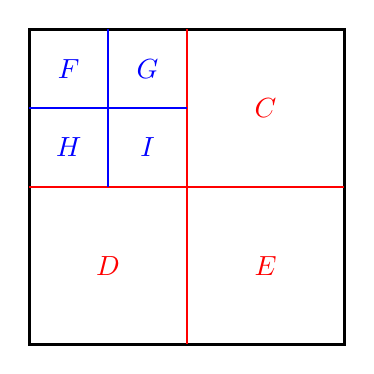
\begin{tikzpicture}
      \draw[very thick] (-2,2) rectangle (2,-2);
      \draw[thick, red] (0,2) -- (0,-2);
      \draw[thick, red] (-2,0) -- (2,0);
      \draw[thick, blue] (-1,2) -- (-1,0);
      \draw[thick, blue] (-2,1) -- (0,1);
      \node at (1,1) {$\textcolor{red}C$};
      \node at (-1,-1) {$\textcolor{red}D$};
      \node at (1,-1) {$\textcolor{red}E$};
      \node at (-1.5,1.5) {$\textcolor{blue}F$};
      \node at (-.5,1.5) {$\textcolor{blue}G$};
      \node at (-1.5,.5) {$\textcolor{blue}H$};
      \node at (-.5,.5) {$\textcolor{blue}I$};
    \end{tikzpicture}\hspace{1.5cm}
    \begin{tikzpicture}
      \Tree [.$A$ [.$\textcolor{red}B$ $\textcolor{blue}F$ $\textcolor{blue}G$ $\textcolor{blue}H$ $\textcolor{blue}I$ ] $\textcolor{red}C$ $\textcolor{red}D$ $\textcolor{red}E$ ]
      \node at (0,-3) {};
    \end{tikzpicture}          
    \caption{Space Partitioning mit Quadtrees}  
    \label{04spdgquadtree}      
\end{figure}

\subsection{Platzierung der Räume und Korridore}
Ausgehend von einer in einer mittels Space Partitioning erstellten Baumstruktur vorliegenden Partitionierung einer rechteckigen Fläche können nun Räume in den Partitionen platziert werden. Da die Partitionen zunächst direkt aneinander anliegen, werden die Räume mit einem durch Parameter beschränkten, zufällig gewählten Abstand zu der linken, rechten, oberen und unteren Begrenzung platziert. Nach der Platzierung der Räume wird der Baum traversiert, um Räume durch Korridore miteinander zu verbinden. Dazu wird in jedem Knoten ein Korridor generiert, der zwei Räume in den Partitionen der Teilbäume der Kinder miteinander verbindet. Der Korridor verläuft dabei durch eine in dem Knoten gespeicherte Unterteilungsebene, wodurch sichergestellt wird, dass Korridore sich nicht überschneiden. Ein Beispiel für einen prozedural generierten Dungeon mit zugehörigem $k$-d-Baum ist in Abbildung \ref{04spdgdungeon} gegeben. Der blau markierte Korridor wurde beispielsweise im Knoten $0$ platziert.
\begin{figure}[h]
    \centering
    \begin{tabular}{cc}
        \begin{minipage}{.4\textwidth}
            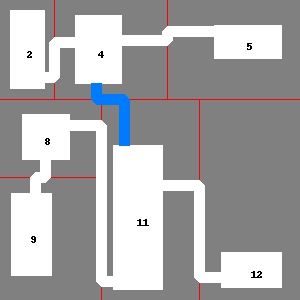
\includegraphics[width = 0.8\textwidth]{resources/img/sp_ex_l3.jpeg}
        \end{minipage}
            &\begin{minipage}{.4\textwidth}
                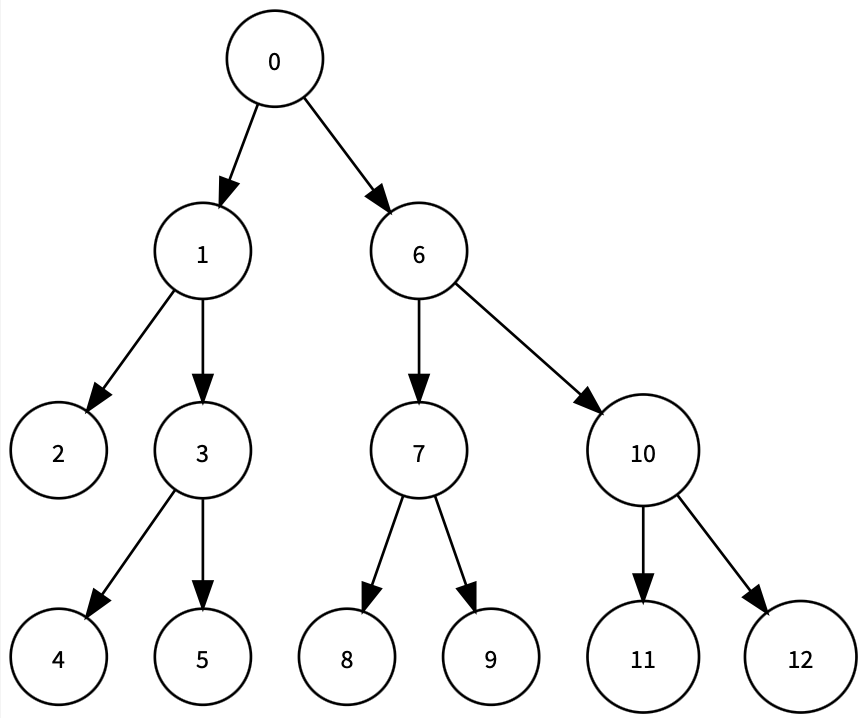
\includegraphics[width = 0.8\textwidth]{resources/img/sp_ex_tree.png}
            \end{minipage}
    \end{tabular}
\caption{Prozedural generierter Dungeon mit $k$-d-Baum}
\label{04spdgdungeon}
\end{figure}